\documentclass[UTF8,fontset=windowsnew]{ctexart}
\usepackage{amsmath}
\DeclareMathOperator*{\uint}{\scalerel*{\rotatebox{8}{$\!\scriptstyle\int\!$}}{\int}}
  \usepackage{scalerel}
\usepackage{hyperref}
\usepackage{graphicx}
\usepackage{xcolor}
\usepackage[left=2cm,right=2cm, top=2cm, bottom=2cm]{geometry}
\usepackage{fancyhdr}
  \pagestyle{fancy}
  \fancyhf{}
  \rhead{\large{\emph{考核系统}}}
  \setlength{\headheight}{20pt}
  \rfoot{\thepage}
\usepackage{enumitem}
\usepackage{tikz}
  \newcommand*\circled[1]{\tikz[baseline=(char.base)]{\node[shape=circle,draw,inner sep=2pt] (char) {#1};}}
  \newcommand{\RomanNumeralCaps}[1]{\MakeUppercase{\romannumeral #1}}
\usepackage{multicol}

\begin{document}
\songti

\section{需求}
\subsection{原始需求}
需要对每个被考核人进行工作量计算。
\begin{enumerate}[label=\protect\circled{\arabic*}]
    \item 工作量计算
    \item 计算过程图像化展示
    \item 用户管理
\end{enumerate}
\subsection{需求分析}
\subsubsection{工作量计算}
\begin{equation}
  C=\frac{1}{N}\sum_{i-1}^NC_i\label{eq:main}
\end{equation}
$C_i=\frac{W_i}{S_i}$为总工作量,$N$为考核项目数量,$W_i$为考核项目完成量,$S_i$为标准任务量。\par
\subsubsection{图像化展示}
将各项参数的组成部分图像化
\subsubsection{用户管理}
允许被考核人亲自上传各个表格
\section{被考核人}
被考核人应由工号辨别,如允许以姓名辨别,应处理重名。\par
每个被考核人属于一种岗位类型:\par
\begin{itemize}
  \item 教学科研岗
  \item 教学岗
  \item 科研岗
\end{itemize}
每个岗位类型分10级,不同等级对应不同的基准工作量和总任务量。
\section{工作量计算标准}
每种考核方向的比重相同,以恰好完成基准工作量为1,如必要项未完成,为0;如非必要项未完成,按比例扣分;如超标完成,按比例加分。\par
完成每种考核后按\autoref{eq:main}计算总分。\par
\section{产品介绍}
由于工期原因,仅需求\circled{1}可以保证完成;如一切顺利,需求\circled{2}可以数字的形式显示,图像化无法完成;需求\circled{3}确定无法按期完成。\par
\subsubsection{基本架构}
\begin{figure}[h]
  \centering
  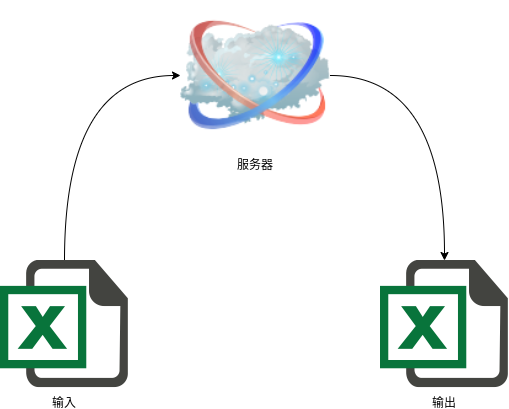
\includegraphics[width=.5\textwidth]{image/struc.png}
  \caption{基本架构}
  \label{fig:struc}
\end{figure}
如\autoref{fig:struc}所示,本产品的基本模式为服务器-客户端模式。\par
\subsection{服务器}
服务器采用Node.js/Express.js/Pug技术,可在Windows/Linux平台上运行。\par
服务器的运行依赖于Nodejs和npm。\par
默认端口为10000。\par
如果需要,可以提供服务器的源代码。\par
测试服务器的地址为\url{http://34.94.165.54:10000/}\par
测试服务器预计可以提供服务到2020年9月。期间如果系统出问题可以保证24小时内解决。
\subsection{客户端}
本产品的客户端为任何浏览器,支持IE 8+, Chrome, Firefox等主流浏览器。如果网页显示出现问题建议更换浏览器后重试。\par
界面:\par
\begin{figure}[h]
  \centering
  
\includegraphics[width=.5\textwidth]{image/client.png}
  \caption{主页面}
  \label{fig:client}
\end{figure}
如\autoref{fig:client}所示,主界面拥有4个链接。\par
\begin{itemize}
  \item [选择表格] 点击该项会弹窗,请选择需要上传的表格
  \item [使用本系统前请阅读此文] 该项为本文的链接
  \item [下载模板表格] 点击该项会下载模板输入表格,请根据模板表格的结构修改输入数据
  \item [上传表格] 点击该按钮会上传输入表格并开始计算。由于输入文件较复杂,需要花费较长时间。请耐心等待10秒。
\end{itemize}
\subsection{输入}
\url{http://34.94.165.54:10000/template}为模板输入文件。其中有12个表格。每个表格有若干列数据列。数据列以外的列不会影响计算,可以随意编辑。\par
数据列第一行不允许改动,否则系统无法识别数据。其它列没有限制。\par
数据列每一列皆有特定的规范,具体请见模板中每一页的注释。\par。
请尤其注意,各表中姓名的识别方式不同,如果姓名的格式错误可能导致该行数据无法识别。
\section{疑问}
以下是对输入数据和算法的疑问。
\begin{enumerate}
  \item 研究生课程是否计入教学课时考核?如是,请提供研究生课程的课时
  \item 课程序号和课程代码哪个是唯一识别码?
  \item 请提供班主任和课程设计的数据
  \item 

  \item 有些表格只有姓名没有工号,为防止重名,建议在每个输入表格中加入工号一栏。如已采用其它处理重名的手段,请告知。
  \item 请提供精确到日的聘期,如2017年1月1日到2019年12月31日。
  \item 必须完成项如果未完成,会对该项分数和总分产生什么影响?如该项分数是否归零,总分是否归零
  \item 如果部分完成了非必须完成项,基本原则是不是按比例扣分?如2级教学科研岗要求到款120万元,实际到款60万,该项分数是否为0.5?
  \item 如果有一项超标完成,基本原则是不是线性加分?如2级教学科研岗到款240万经费,该项分数是否为2?
  \item ``教学课时''考核中,``每年''字样和学年度学期间的对应关系。如2017年等于2016-2017学年第二学期加上2017-2018学年第一学期。
  \item ``教学课时''考核中,如何判断一门本科生课程是否为核心课程?
  \item ``教学课时''考核中,课程设计、班主任数据的来源与折算成课时的算法。如一个学期的班主任折算成本学期多少课时。
  \item 《2016-2019年科创项目.xlsx》中,是否按申报年份一列判断是否在聘期内?
  \item 《2016-2019年科创项目.xlsx》中,指导大学生科创折算成指导老师课时的算法。如2017年申报的一项科创项目折算成2017年多少课时
  \item ``教学课时''考核中,2级教学科研岗的基准要求每年上1门课,至少64课时。若每年承担2门课,共64课时,该项分数为1.5还是1?
  \item ``教学课时''考核中,2级教学科研岗若每年承担2门课,共128课时,该项分数为2还是4?
  \item ``教学课时''考核中,2级教学科研岗若2017和2018年各承担1门课,64课时,但19年没有上课,在不考虑其它项目折算课时的前提下,该项考核是否算0.66?
  \item ``教学课时''考核中,2级教学科研岗若2016-2017学年第二学期上了一门课共64课时,在2017-2018学年第一学期没有上课,2017年该项的分数是否为1?
  \item ``聘期内教学改革''考核中,判断是否完成本专业教学任务的依据
  \item ``聘期内教学改革''考核中,判断是否作为核心课程骨干教师的依据
  \item ``聘期内教学改革''考核中,判断是否引领教学改革的依据
  \item ``聘期内教学改革''考核中,判断是否引领实验教学平台建设的依据
  \item ``聘期内教学改革''考核中,判断是否引领课程建设的依据
  \item ``聘期内教学改革''考核中,判断是否引领教材建设的依据
  \item ``聘期内教学改革''考核中,国家级优秀教材奖的数据来源与判断依据
  \item ``聘期内本科实验教学建设''考核的数据来源与判断依据
  \item ``聘期内科研项目数''考核中,新增科研项目是按立项日期算还是按研究开始日期算?
  \item ``聘期科研项目经费到款''考核中如果有15年立项的项目,19年到款,是否算入考核?
  \item 《经费到账数据导出.xls》中的校管理费等金额列的单位是否都统一为(万元)?
  \item 10级教学科研岗要求聘期经费到账60万元或聘期内主持国家级项目。若15年立项国家级项目,至今仍在主持,在无经费到款的前提下,``聘期内科研项目''考核分数是否算1?
  \item 如果10级教学科研岗15年立项国家级项目,18年项目结束,在无经费到款的前提下,``聘期内科研项目''考核分数是否算1?
  \item 如果10级教学科研岗既到款经费60万元,又主持了一项国家级项目,``聘期内科研项目''考核是否算2?
  \item 如果10级教学科研岗到款经费120万元,未主持国家级项目,``聘期内科研项目''考核是否算2?
  \item 如果10级教学科研岗到款经费0元,主持国家级项目2项,``聘期内科研项目''考核是否算2?
  \item ``S4''考核中如何判断一篇论文是不是教学研究论文?又如何判断是不是科研学术论文?
  \item ``S4''考核中成果奖的数据来源与等级、排名的判断依据
  \item ``S4''考核中精品课程的数据来源和等级的判断依据。(排1)和(前2)的意义
  \item ``S4''考核中出版教材的数据来源和(前3)的意义
  \item ``S4''考核中学生创新竞赛或学科竞赛的数据来源与等级判断依据
  \item ``S4''考核中标红的项目有何特殊
  \item ``S4''考核中教学成果奖的数据来源与等级的判断依据
  \item ``S4''考核中如果超标完成,如教学科研岗2级既完成了\circled{1}又完成了\circled{2},该项评分是否为2
  \item ``科研成果''考核中,《论文数据导出.xls》中的收录类别一列是否为SCI的判断标准?具体哪几种收录类别为SCI?
  \item ``科研成果''考核中,专利成果转化的数据来源
  \item ``科研成果''考核中,如何判断专利授权在``聘期内''?
  \item ``科研成果''考核中,专利一项中(前3)的意义?
  \item ``科研成果''考核中,教材、专著、编著之间的关系?
  \item ``科研成果''考核中,出版专著中的(前3)的意义?
  \item ``科研成果''考核中,科研成果奖的数据来源与等级判断依据
  \item ``集体工作''考核的数据来源与判断依据
\end{enumerate}
\end{document}
